\documentclass[final,hyperref={pdfpagelabels=false}]{beamer}
\usepackage{grffile}
\mode<presentation>{\usetheme{QUB}}
\usepackage[english]{babel}
\usepackage[latin1]{inputenc}
\usepackage{amsmath,amsthm, amssymb, latexsym}
\usepackage[scaled=0.98]{helvet}
%\usepackage{times}\usefonttheme{professionalfonts}  % obsolete
%\usefonttheme[onlymath]{serif}
\boldmath
\usepackage[orientation=landscape,size=a1,scale=1.0,debug]{beamerposter}
\usepackage{wrapfig}
\usepackage{comment}
% change list indention level
\setdefaultleftmargin{5em}{}{}{}{}{}


%\usepackage{snapshot} % will write a .dep file with all dependencies, allows for easy bundling

\usepackage{array,booktabs,tabularx}
\newcolumntype{Z}{>{\centering\arraybackslash}X} % centered tabularx columns
\newcommand{\pphantom}{\textcolor{ta3aluminium}} % phantom introduces a vertical space in p formatted table columns??!!
\usepackage{parcolumns}

\listfiles

%%%%%%%%%%%%%%%%%%%%%%%%%%%%%%%%%%%%%%%%%%%%%%%%%%%%%%%%%%%%%%%%%%%%%%%%%%%%%%%%%%%%%%
\graphicspath{{figures/}}
 
\title{\huge Towards Distributed, Behaviour-Based Trust for Autonomous Submarine Teams}
\author{Andrew Bolster, Prof. Alan Marshall, Prof. Jean-Guy Fontaine }
\institute[QUB]{Electronics Communications and Information Technology Institute, Queens' University Belfast, UK}
\date[27/02/13]{Febuary 27th, 2013}

%%%%%%%%%%%%%%%%%%%%%%%%%%%%%%%%%%%%%%%%%%%%%%%%%%%%%%%%%%%%%%%%%%%%%%%%%%%%%%%%%%%%%%
\newlength{\columnheight}
\setlength{\columnheight}{55cm}

\def\colwidth{0.25\linewidth}

\usecaptiontemplate{
\small
\structure{\insertcaptionname~\insertcaptionnumber:}
\insertcaption
} 
%%%%%%%%%%%%%%%%%%%%%%%%%%%%%%%%%%%%%%%%%%%%%%%%%%%%%%%%%%%%%%%%%%%%%%%%%%%%%%%%%%%%%%
\begin{document}
\begin{frame}[fragile]
  \begin{columns}[t]
    % ---------------------------------------------------------%
    % Set up a column 
    \begin{column}{\colwidth}
      \begin{beamercolorbox}[center,wd=\textwidth]{postercolumn}
        \begin{minipage}[T]{.98\textwidth}  % tweaks the width, makes a new \textwidth
          \parbox[t][\columnheight]{\textwidth}{ % must be some better way to set the the height, width and textwidth simultaneously
            % Since all columns are the same length, it is all nice and tidy.  You have to get the height empirically
            % ---------------------------------------------------------%
            % fill each column with content            
%%%%%%%%%%%%
            \begin{block}{Introduction}
              \emph{Aim of project}: To use physical behaviours and observations to assess trust within a mobile, marine, ad-hoc networks without wasting communications time / energy

              \vspace{\lineskip}
              \begin{itemize}
                \item Small fleets of AUVs (\emph{Autonomous Underwater Vehicles}) will be expected to operate in isolated environments.
                \item This requires an auditable sense of trust within the remote intra-fleet communications networks, incorporating
                  \begin{itemize}
                    \item Communications Activity
                    \item Mission Suitability/Capability
                    \item Behavioural Monitoring
                  \end{itemize}
                \item The use of centrally coordinated trust models presents a single point of failure.
                \item Verifiably secure direct communications in marine environments are expensive and time consuming; adopting a decentralised form of trust assurance will reduce these costs by localising the per-node security environment.
              \end{itemize}
            \end{block}
%%%%%%%%%%%%
\iffalse
            \begin{block}{Context Areas}
              \begin{itemize}
                \item This Behaviour monitoring is the subject of the current work and touches on many areas
                \begin{itemize}
                  \item Distributed Trust
                  \item Grey-Theory Analysis
                  \item Anomaly Detection and Identification
                  \item Underwater Localisation
                  \item Flock Simulation
                  \item Collaborative Path Planning
                  \item Iterative Principal Component Analysis
                  \item \dots and more not yet covered
                \end{itemize}
              \end{itemize}
            \end{block}
\fi
%%%%%%%%%%%%
              \begin{block}{Trust}
                  Trust is:
                  \begin{itemize}
                    \item an assessment of the likelihood of an entities action upon request
                    \item a belief on the reliability of an entity
                    \item based on both direct and indirect historical experience
                  \end{itemize}

                  Individual trust opinions are shared within the team concerning a range of activities:
                  \begin{itemize}
                    \item Transmission Relaying (Local and/or Backhaul)
                    \item Position Relaying
                    \item Reporting Accuracy
                  \end{itemize}

                  These Trust opinions also apply to extra-fleet entities, such as surface platforms, submarine comms links, and coastal stations, allowing the fleet to collaboratively form an opinion of these actors.
                  \begin{wrapfigure}{r}{0.45\textwidth}
                    \vspace{-20pt}
                    \begin{center}
                      \includegraphics[width=0.4\textwidth]{../../figures/trust_explanation.dot}
                    \end{center}
                    \vspace{-30pt}
                    \caption{Direct and in-direct trust}
                    \vspace{-20pt}
                  \end{wrapfigure}
                  In this context, Trust is implied to be both the trust between nodes within a fleet, and the continuous assessment of trust of between the fleet and extra-fleet entities such as operators and fleet-commanders, providing an ongoing assessment of the likelihood of success of a particular mission.
                  
            \end{block}
%%%%%%%%%%%%
            \begin{block}{Behaviour}
              To develop a trust scheme based on operational behaviours, those behaviours must be investigated to assess what metrics to use for trust and reputation modelling. 

              \vspace{0.5\baselineskip}

              Behaviours currently under investigation include:
              \begin{itemize}
                \item \emph{Waypointing} - Attraction to a point or a chain of points, providing pre-described patrol networks
                \item \emph{Surveying} - Fleets can be tasked to provide one-shot, or persistent coverage of an area of the environment
                \item \emph{Dynamic Constraint} - Repulsion from a series of points, analogous to sea-borders or shipping lanes.
              \end{itemize}

              \vspace{0.5\baselineskip}

              Potentially Exploitable Behaviours not yet developed include:
              \begin{itemize}
                \item \emph{Capacity Based Homing} - For instance for refuelling or resupply, the fleet (or individuals within the fleet) can break 
                  away to a static or mobile \emph{mothership} and return to the estimated fleet position
                \item \emph{Dynamic Communications Maintenance} - The fleet can adjust to changing communications environments by factoring metrics such 
                  as packet loss into flocking model, closing together in poor communications environments and expanding in good environments.
              \end{itemize}
            \end{block}
%%%%%%%%%%%%
          }
        \end{minipage}
      \end{beamercolorbox}
    \end{column}
    % ---------------------------------------------------------%
    % end the column

    % ---------------------------------------------------------%
    % Set up a column 
    \begin{column}{\colwidth}
      \begin{beamercolorbox}[center,wd=\textwidth]{postercolumn}
        \begin{minipage}[T]{.98\textwidth} % tweaks the width, makes a new \textwidth
          \parbox[t][\columnheight]{\textwidth}{ % must be some better way to set the the height, width and textwidth simultaneously
            % Since all columns are the same length, it is all nice and tidy.  You have to get the height empirically
            % ---------------------------------------------------------%
            % fill each column with content
            
%%%%%%%%%%%%
\iffalse
            \begin{block}{Flocking Behaviour Fundamentals (Boid-like)}
              \begin{columns}[T]
                \begin{column}{.70 \textwidth}
                  \begin{itemize}
                    \item Cohesion
                      \begin{equation}
                        F_{j,C}= F_A\left(p_j, \frac{1}{N}\sum\limits_{\forall i \ne j}^N{p_i}, d_{max}\right)
                      \end{equation}
                    \item Repulsion
                      \begin{equation}
                        F_{j,H}= \sum\limits_{\forall i \ne j}^N F_R\left(p_j, p_i, d_{max}) \big| d_{max}>\|p_i-p_j\|\right)
                      \end{equation}
                    \item Alignment
                      \begin{equation}
                        F_{j,CA}= \frac{1}{N}\cdot\left(\sum\limits_{\forall i \ne j}^N \hat{v_i}\right) 
                      \end{equation}
                    \end{itemize}
                \end{column}
                \begin{column}{.25\textwidth}
                  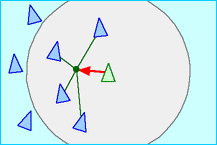
\includegraphics[width=0.9\textwidth]{figures/flocking_cohesion.gif}
                  \vspace{\baselineskip}
                  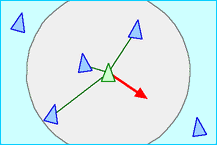
\includegraphics[width=0.9\textwidth]{figures/flocking_separation.gif}
                  \vspace{\baselineskip}
                  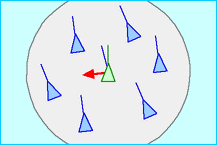
\includegraphics[width=0.9\textwidth]{figures/flocking_alignment.gif}
                \end{column}
              \end{columns}
              \vspace{\baselineskip}
              Where $F_A$ is a scaled vector attraction function, and $F_R$ is an equivalent repulsion function
            \end{block}
\fi
%%%%%%%%%%%%
            \begin{block}{Simulation Framework}
              Bespoke Simulation framework consisting of three modules:
              \begin{itemize}
                \item \texttt{Aietes} : the original base behavioural simulator, performing agent-based modelling of the motions of AUV's within an 
                  environment
                \item \texttt{Bounos} : a collection of data processing and collation functions.
                \item \texttt{Ephyra} : a GUI visualisation (and later, control) system for both Aietes and Bounos (See Fig~\ref{fig:Ephyra})
              \end{itemize}

              \vspace{0.5\baselineskip}

              It is highly flexible, allowing for:
              \begin{itemize}
                \item Arbitrary node configurations (both in terms of physical and communications capabilities)
                \item Generically Based on the REMUS 100 configuration and physical model, but extendible to other dynamics
                \item Support for runtime and \emph{a-posteriori} statistical analysis with numpy/scipy/pandas
                \item Componentised Behaviour network, with a Boid-like collaborative control path base behaviour (flocking)
                \item Integration to the SUNSET emulation platform, allowing for rapid integration to real equipment
              \end{itemize}
              \vspace{\lineskip}
              \begin{figure}
                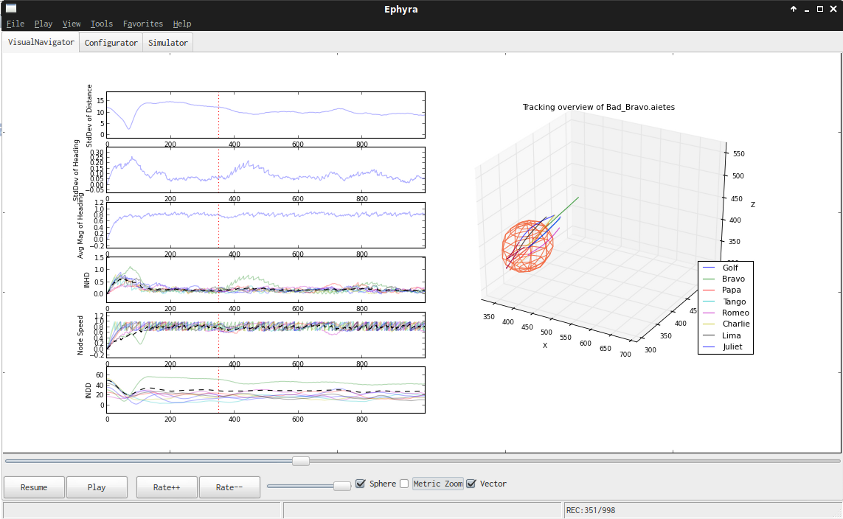
\includegraphics[width=0.9\textwidth]{figures/ephyra_vis}
                \caption{The Ephyra visualiser built with WxPython allows for rapid modelling and analysis of multi-dimensional vector data, in this case showing a interactive real-time 3D model of the fleet positions and trails, as well as overlay information on individual and fleet behaviours, and on the left, fleet- and node- level metrics plotted over time.}
                \label{fig:Ephyra}
              \end{figure}
            \end{block}     
%%%%%%%%%%%%
             \begin{block}{Proof Of Concept}
              \begin{itemize}
                \item Using a simple misbehaviour such as a rogue AUV following the fleet (and the fleet rules) without knowledge of the mission 
                  specification as a Theoretical Proof of Concept allows for rigorous analysis of research options.
                \item Taking a selected metric (Inter Node Distance Deviation \emph{INDD}), it is shown that detection is possible and reliable (after a suitable 
                  stabilisation time).
                \item This metric is isolated from other analysed metrics as shown in Figure ~\ref{fig:Bad_Bravo_Comparison}, where \emph{INDD} 
                  is the only consistently observable differentiating metric between normal behaviour and rouge behaviour.
                \item It is also shown that before stabilisation, it is nearly impossible to differentiate.
                \item Additional related metrics such as the Inter Node Heading Deviation \emph{INHD} and the simple Speed of the nodes are slightly 
                  discriminating, but are not as consistent as \emph{INDD}.
                \item All of the current metrics are real-time computed and require no \emph{a-priori} knowledge of the fleet, but require a high degree of 
                  accuracy in the positional and (hence) velocity spaces.
              \end{itemize}
            \end{block}   
%%%%%%%%%%%%

          }
        \end{minipage}
      \end{beamercolorbox}
    \end{column}
    % ---------------------------------------------------------%
    % end the column

    % ---------------------------------------------------------%
    % Set up a column 
    \begin{column}{\colwidth}
      \begin{beamercolorbox}[center,wd=\textwidth]{postercolumn}
        \begin{minipage}[T]{.98\textwidth} % tweaks the width, makes a new \textwidth
          \parbox[t][\columnheight]{\textwidth}{ % must be some better way to set the the height, width and textwidth simultaneously
 
%%%%%%%%%%%%
            \begin{block}{Analysis}
              Taking two simulated fleets in a simple patrol mission, one with a malicious node, and comparing the metrics of:
              \begin{itemize}
                \item \emph{INHD}: Inter Node Heading Deviation, or the per-node deviation from the fleet-average velocity vector
                \item \emph{Node Speed}: The Magnitude of Velocity of each node
                \item \emph{INDD}: Inter Node Distance Deviation, or the normalised deviation between the inter-node distance matrices from the perspective of each node
              \end{itemize}
              \begin{figure}
                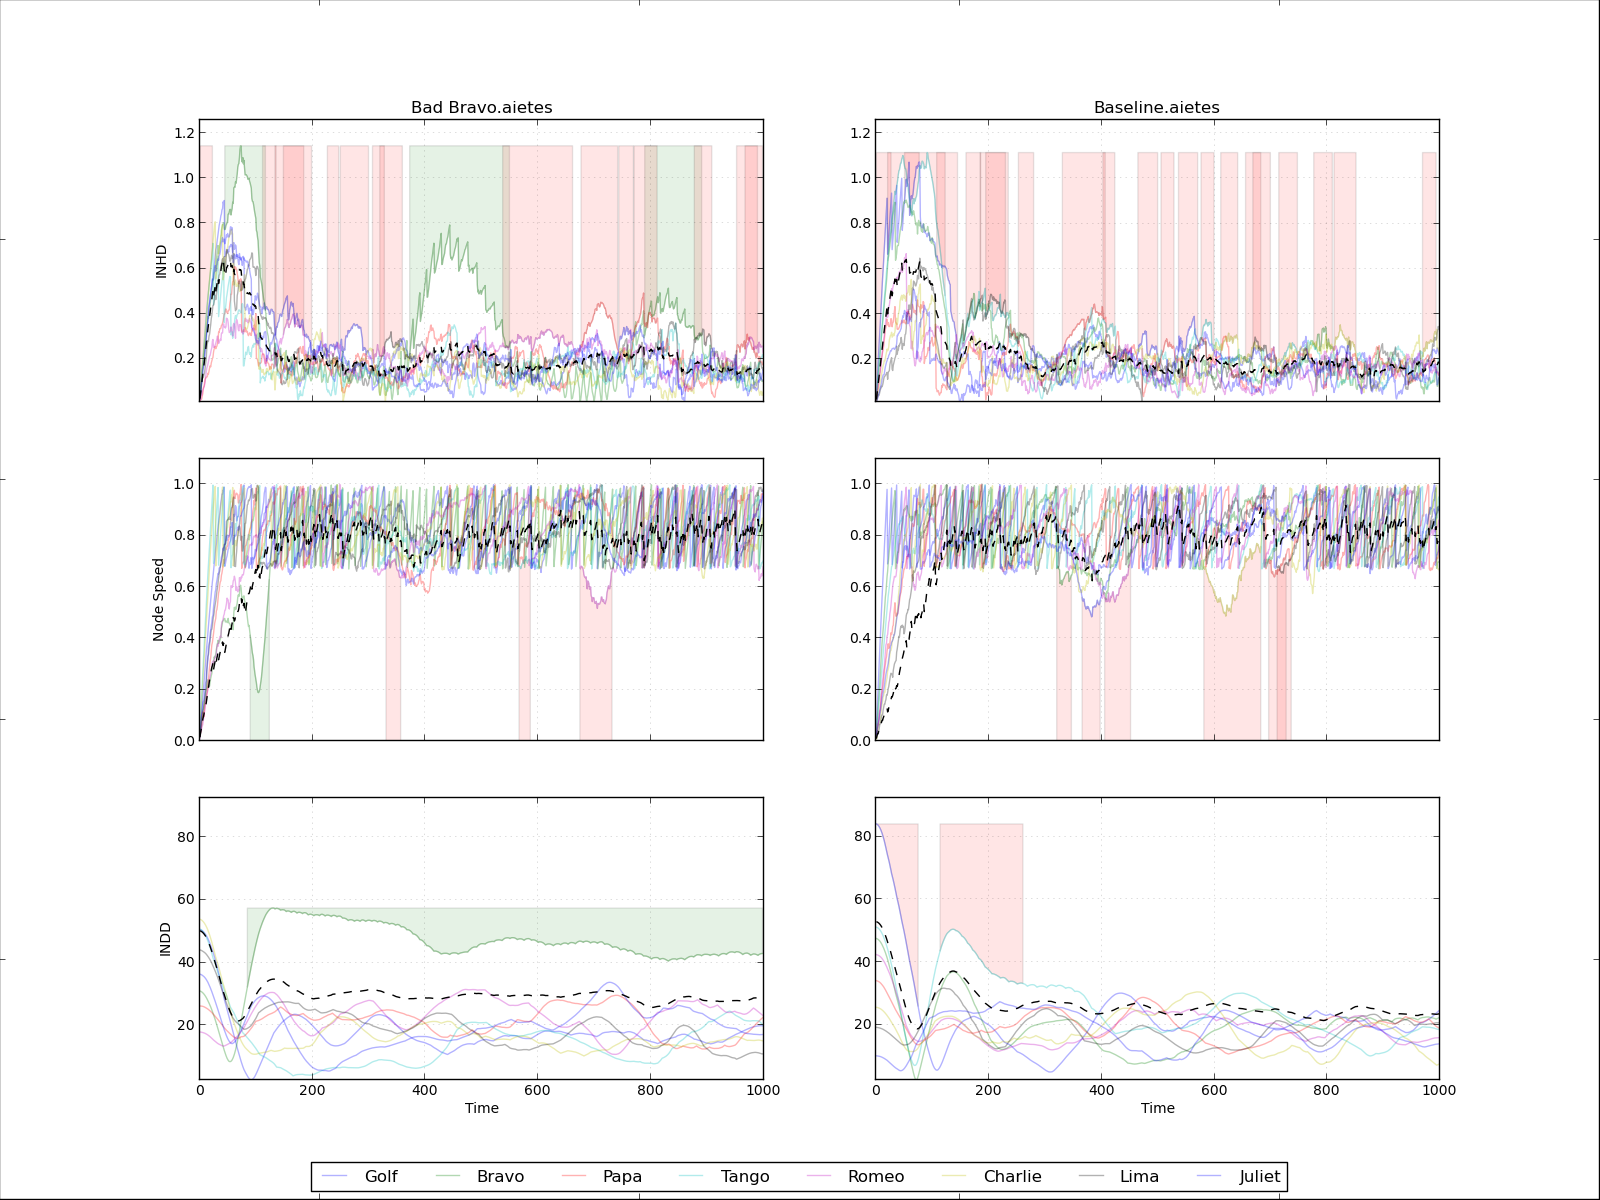
\includegraphics[width=0.9\textwidth]{figures/Bad_Bravo_Comparison_With_Detection}
                \caption{Metric Comparison chart showing each metric (vertically) for each simulation run (horizontally) where the left-hand-side charts are have a malicious node (Bravo). The black dashed lines represent the fleet-average value for each metric. Highlighted sections of the graph highlight Positive detections (Green) and False Positive Detections (Red)}
                \label{fig:Bad_Bravo_Comparison}
              \end{figure}
              
              \emph{INDD} is clearly a obvious candidate for a trust assessment metric, but looking at \emph{INHD} values after around 400-600 seconds of simulation time; an anomaly is clearly being detected. 

              \vspace{\baselineskip}

              In addition, \emph{Bravo} node (the Green Line) is clearly an outlier in terms of \emph{INHD} and \emph{Node Speed} in the earliest sections of the graph, at which point nothing appears to be out of the ordinary in \emph{INDD}. This implies that a fusion of metrics would be more effective than a simple detection envelope on a single metric.

              \begin{figure}
                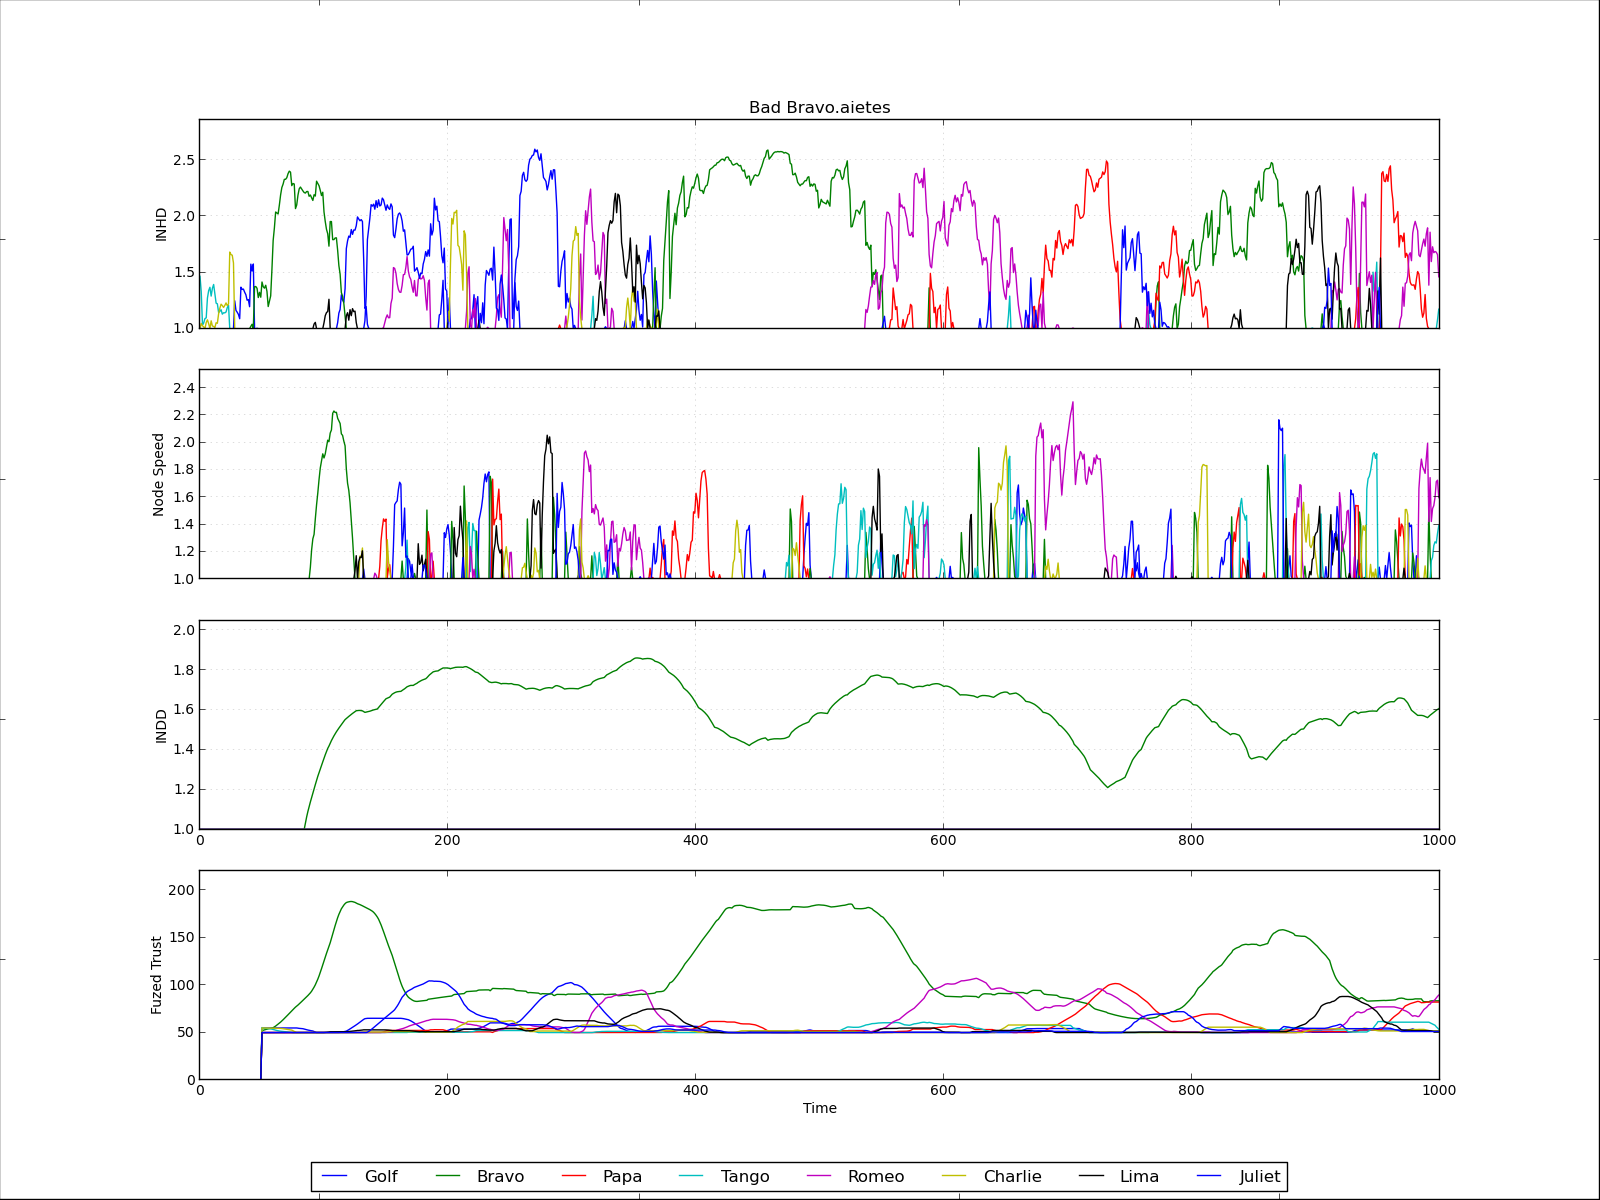
\includegraphics[width=0.9\textwidth]{figures/Bad_Bravo_Fusion}
                \caption{This chart shows the deviation ratios from fleet-mean for each metric in Fig. ~\ref{fig:Bad_Bravo_Comparison}, and subsequently takes an (unweighted) sliding-window, cumulative product, as a PoC combined trust metric}
                \label{fig:Bad_Bravo_Fusion}
              \end{figure}


            \end{block}
        
%%%%%%%%%%%%
          }
          % ---------------------------------------------------------%
          % end the column
        \end{minipage}
      \end{beamercolorbox}
    \end{column}
    % ---------------------------------------------------------%

    % ---------------------------------------------------------%
    % Set up a column 
    \begin{column}{\colwidth}
      \begin{beamercolorbox}[center,wd=\textwidth]{postercolumn}
        \begin{minipage}[T]{.98\textwidth} % tweaks the width, makes a new \textwidth
          \parbox[t][\columnheight]{\textwidth}{ % must be some better way to set the the height, width and textwidth simultaneously
            % Since all columns are the same length, it is all nice and tidy.  You have to get the height empirically
            % ---------------------------------------------------------%
            % fill each column with content

%%%%%%%%%%%%

            \begin{block}{Analysis Cont.}
              However, looking at the Baseline data (Right side of Figure ~\ref{fig:Bad_Bravo_Comparison}), it's clear that these metrics are not infallible, as is demonstrated by the number of relatively short-lived false positives.

              \vspace{\baselineskip}

              Figure ~\ref{fig:Bad_Bravo_Fusion} demonstrates a simple unweighted trust fusion, where deviations in individual metrics are additively combined to generate a coarse Trust Value. It's clear from the massive impact of \emph{INDD} on the fused value is a problem that needs to be solved, as not all potential misbehaviours will be so evident in this single metric.
            \end{block}
            \begin{block}{Future Work}
              \begin{itemize}
                \item PoC demonstrates that it is relatively simple to detect and identify misbehaving if an observer has all available data to a suitable degree 
                  of accuracy and timeliness
                \item Next steps are to develop a suite of misbehaviours and analyses to construct an agnostic trust framework, combining these 
                  multiple analysis metrics via Gray Theory so as to provide detection, discrimination, and identification of the full range of 
                  potential misbehaviour/failure states
                \item Once this framework is completed, the data-availability will be iteratively stripped back to approach the realistic communications and sensor environment, and the failure state of the framework will be assessed
              \end{itemize}
            \end{block}           
%%%%%%%%%%%%
            \begin{block}{Future Applications}
              \begin{itemize}
                \item Due to the high communications, motion, and computation costs, and lack of external location reporting (\emph{e.g. GPS}), 
                  behavioural analysis in the marine environment is particularly difficult, but if successful, can be reliably applied in a wide 
                  variety of fields including but not limited to
                \begin{itemize}
                  \item Self-Driving Cars
                  \item Environmental Survey drones (terrestrial, marine, and aerial)
                  \item Satellite Communications Arrays
                  \item Internet Certificate Authority verification
                  \item Verifiable Distributed Computing
                \end{itemize}
              \end{itemize}              
            \end{block}
%%%%%%%%%%%%
            \begin{block}{Conclusions}
              This research area presents a range of challenges and opportunities within both civil and defence operations; an auditable trust framework for automated marine craft would be a significant enabling factor to the roll-out of more low-maintenance or even ``Fire and Forget'' deployments for persistent patrol/monitoring tasks. 

              \vspace{\baselineskip}

              Related innovations in battery, propulsion, sensor and communications packages will enable small teams of AUVs to remain trusted even outside of in-field communications networks, and can even be used as a Disruption Tolerant Network (DTN) to vastly expand the in-field network with low power communications. These teams could silently patrol independently and only return to a communicative state upon mission-status-change and/or when the team itself detects that it is under attack.

            \end{block}
          }
          % ---------------------------------------------------------%
          % end the column
        \end{minipage}
      \end{beamercolorbox}
    \end{column}
    % ---------------------------------------------------------%
    % end the column   % end the column
  \end{columns}
  \vskip1ex
  \tiny\hfill{Created with \LaTeX \texttt{beamerposter}  \url{http://www.ecit.qub.ac.uk/Research/DigitalCommunications/} \hskip1em}
\end{frame}
\end{document}


%%%%%%%%%%%%%%%%%%%%%%%%%%%%%%%%%%%%%%%%%%%%%%%%%%%%%%%%%%%%%%%%%%%%%%%%%%%%%%%%%%%%%%%%%%%%%%%%%%%%
%%% Local Variables: 
%%% mode: latex
%%% TeX-PDF-mode: t
%%% End:
